\chapter{Wireless Sensor Network Architecture Design}\label{chap:arch}
	In this chapter, we explain our proposed network architecture that uses local and global knowledge to make informed routing decisions and to classify sensed data within the network. Our approach, K-HAS, uses a three-tiered, hierarchical approach with each subsequent tier providing increased knowledge processing capabilities. 

	We aim to show that sensors capable of processing knowledge will provide a more efficient network and be able to prioritise the delivery of interesting sensed data. We also believe that human input is a valuable way for such a network to learn about classifications it has made correctly, and incorrectly, and use that knowledge to inform future classifications. To prove this, we have developed an architecture that uses different levels of knowledge processing throughout the network, the Knowledge-based Hierarchical Architecture for Sensing (K-HAS).

	The rest of this chapter is structured as follows. Section \ref{arch:khas} outlines the main aims of K-HAS and what it is capable of that typical sensor networks are not. Section \ref{arch:tech} details the software and data standard choices we made for our implementation of K-HAS. Section \ref{arch:walk} provides a sample walkthrough of K-HAS, relating to our motivating scenario and Section \ref{arch:conc} concludes the chapter.

	\begin{figure}[h]
			\centering
			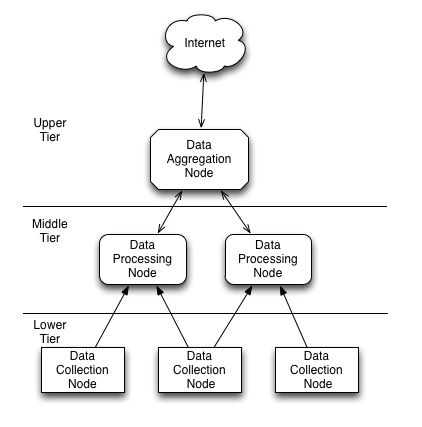
\includegraphics[width=0.65\textwidth]{Chap4/figures/khasarch} 
			\caption{Overview of the K-HAS Architecture}
			\label{arch:khas:arch}
			\end{figure}
	
	\section{K-HAS}\label{arch:khas}
		K-HAS has been designed as an architecture for WSNs that uses knowledge to classify sensed data and adapt to changes in the structure of the network. By pushing knowledge bases out to the edge of the network, all nodes in the network have some awareness of the data they are sensing, as well as how important it is, based on the current projects that the network is involved in. This is achieved by using rules with different levels of granularity based on the knowledge processing capabilities of that tier. Figure \ref{arch:khas:arch} shows a high level overview of K-HAS, showing the flow of data from each tier.
	
	
	\subsection{Data Collection}\label{khas:dc}
	The data collection (DC) tier is very similar to sensor nodes commonly used in a WSN, using hardware that has similar, limited processing power and storage to nodes such as: the I-Mote and Waspmote. These DC nodes are deployed at the edge of the network and tasked with sensing their environment, pre-processing the sensed data and using each other to relay data to the next tier.

	DC nodes are capable of performing processing on data, such as the time it was recorded and its size, but their limited knowledge processing capabilities allow them to have an increased battery life and reduced size, making them suitable for a variety of deployments as they can be integrated easily with existing devices (i.e. cameras) and be easily disguised, or hidden.

	\subsubsection{Knowledge Base}
	Reduced knowledge processing capabilities and low memory restrict the knowledge that these nodes can hold and they are limited to a static knowledge base that is encoded at the time of 	deployment. DC nodes run an operating system designed for embedded devices, the size of the operating system is minimal when compared to an operating system used on modern desktop computers and provides much more limited functionality, such as sleep scheduling, basic filesystem access and the capabilities to run a variation of popular languages. 

	For example, TinyOS \cite{levis2005} is an operating system designed for sensor nodes and uses a dialect of the C language, called nesC, that is optimised for the memory constraints of most sensor nodes. The operating system exposes components that allow basic commands, such as reading from the sensor interface or sending a message. Commands are executed as a request to perform some action and events signal the completion of that action. Intensive tasks, such as data processing, can be scheduled to run at a later time, ensuring that the low-power node remains responsive and preventing any calls from blocking other events.

	The Waspmote nodes, explained in Section \ref{tech:waspmote}, do not run any operating system and any event handling, networking or memory management is performed solely by the single file application that is uploaded to the node through the bootloader. Performing intensive tasks, such as local data processing, can drain the battery of the node, cause it to fill the available memory or even cause the node to go down. DC nodes do not have the safeguards in place that most operating systems and applications do, operational code must be lightweight, responsive and ensure that events do not run for longer than intended. 

	Some nodes within this class do not have the capability to process text files within the file system and, therefore, must have the knowledge added to their operational code. DC nodes only perform simple operations on the properties and content of the data that they sense, such as the time it was recorded, the location and its size. For more complex data, such as images and video, DC nodes do not possess the computational power required to process them and instead use the metadata associated.
	Unlike modern rule engines, these static rules do not use forward chaining and the outcome of one rule does not cause the rules to be fired again. Listing \ref{kb:dcrule} shows an example of some of the rules in the knowledge base and highlights that the core structure of this file is simply a list of if statements that can be executed one after the other. Forward chaining is not used here because processing times need to be kept to a minimum and a chain of rules being fired could easily overwhelm the node. If any rules are fired that suggest the observation may be interesting, it is prioritised through the network and potential classifications are encoded within the observation before it is sent on.

\begin{lstlisting}[breaklines=true, caption={Pseudocode DC Node Rules}, label={kb:dcrule}]
if month of observation is JUNE AND time of observation is between 17:00 and 19:00 and active otter project is TRUE
	add classification to observation(`Potential Otter sighting')
	prioritise observation as interesting
if temperature is 37 AND time of observation is between 01:00 and 05:00 and active leopard project is TRUE
	add classification to observation(`Potential Leopard sighting')
	prioritise observation as interesting
\end{lstlisting}

When the data is recorded by the DC node, the knowledge base is fired and inferences are made about the contents of the data. Each DC node has a static knowledge base loaded onto it before it is deployed, which is based on the local knowledge of the area that it is to be deployed in.  For example, a node deployed on the bank of a river would have a different knowledge base to a node deployed in the fields of a plantation.

Once a trigger has been processed, the data is packaged and then sent on to the Data Processing (DP) node.

	\subsection{Data Processing}\label{khas:dp}
	DP nodes act as cluster heads of the network, serving a subset of all deployed DC nodes. When data is sensed, it is forwarded through all DC nodes to the DP node that is tasked with serving the originating DC node. These nodes have more knowledge-processing capabilities than a DC node and do not perform any direct sensing. 

	Due to the greater capabilities, DP nodes have a much shorter battery life than DC nodes and a network typically consists of fewer DP nodes. These capabilities, such as increased memory and higher processing power, allow DP nodes to run a rule management system (such as Drools \cite{proctor2005drools}), that would not be possible on nodes that run on an OS for embdedded systems, that is able to handle more complex rules and process more than just files, they can perform the same tasks as most modern computers, such as: image processing, audio processing or reading metadata from files that requires extra libraries. When a DP node receives data, it processes everything associated, this includes metadata, the data itself and the inferences made by the DC node. If the DC node has inferred that the data is of a higher priority, then this data is processed first. This is done by prioritising the data at two stages: once it has been received and when it is about to be sent.

	In our current implementation, DP nodes use two different radios, a Zigbee radio to allow long range communication from DC nodes and a Wi-Fi radio that provides short range communication that allows for higher data rates.

	\subsubsection{Knowledge Base}
	In our motivating scenario the network is image-based, this means that the DP node would perform image processing, as well as processing the image metadata. The increased knowledge processing capabilities allow DP nodes to run rules dynamically, learning from the sensed data and providing classifications that change based on changes in the environment. For example, if a DP node has not seen an elephant before, and it is not aware of the object in the image, then it will await a human classification. The node will then record the time period that it receives elephant pictures, i.e. June to July, and become more alert the following year. Similarly, the node will know not to look for pictures of nocturnal animals during the day. This local knowledge allows processing power to be saved and, thus, time; this ensures that the processing of sensed data is optimised as much as possible in order to reduce the time it spends in the network.
	
	% The rule engine used in our current implementation is Drools, a Java based rule engine that allows for rules to be defined in \textit{.drl} files and these can be loaded dynamically into a knowledge base. This flexibility allows to be changed on the fly without the need to restart the device, or even require human access, as all of this can be achieved through network communication. 
	The rule engine used should allow for rules to be dynamically inserted into the rule base, so that rules can be updated through network communication.

	Upon receiving sensed data from a DC node, the rule base is fired on the metadata of each file received. If the rules determine that the data is of interest or, in the best case scenario, provides a classification, then the data is packaged and sent on to the Data Aggregation (DA) node.
	
	\subsection{Data Aggregation}
	Placed at the root of the network, these are nodes with the same knowledge-processing capabilities as DP nodes (although they typically have greater memory, processing power and a continuous power source) and would be accessible by users of the network. When DA nodes receive sensed data, it is unpacked and stored with a link to the node that the data originated from. Compared with a standard WSN, these nodes can be compared with a base station, or endpoint.
	
	Any information added by the DP node is parsed and classifications are extracted. If a classification is found, it is stored and the DA node checks for any active projects that contain the classification. If a match is found then all users involved in the project are informed via their preferred method of communication. Using the motivating scenario as an example, the people involved with projects could be researchers and professors and they may be looking for images of leopards, requesting to be informed via Twitter.
	
	All sensed data received, regardless of whether it has been classified, is accessible through a web interface hosted by each DA node. The interface shows all of the sensed data from each deployment, along with the associated classification. More importantly, it allows users to classify the data using a voting system. Users have roles which give them different privileges within the system. Normal users are able to vote and the majority vote is seen to be the current classification. While this is not a necessary feature of a DA node, it does allow the network to utilise the knowledge of human experts to inform future classifications.
	
	However, privileged users are able to confirm a classification and prevent any further votes. Once a classification has been confirmed, it is then sent back to the DP node it originated from. If the classification made by a user is different to the one inferred by the node, then it updates its knowledge base and acknowledges receipt.

	This system is vital in the early stages of deployment as this is used to build up a knowledge base. The more user classifications there are, the more accurate the network will be in the future. After a few months of classifications, K-HAS is then able to use the knowledge base to make more informed classifications, requiring fewer classifications/confirmations from users. The exception to this is sensed data that cannot be matched to the knowledge base.
	
	\subsubsection{Knowledge Base}
	DA nodes do not typically experience the resource constraints that DC and DP nodes must compensate for. Because of this, they hold a global knowledge that contains a history of all observations made by all nodes, as well as the location and deployment times of all nodes in the network. When nodes are deployed, this is updated, by users, to show the location of the node and when it was placed. 

	Every classification sent from DP nodes is stored in a database and contains all information about an observation: date, time, originating node, route taken within the network, location, sensed data, classification of sensed data. They also hold information for all projects running, for example: a project to track elephant movements within the forest. When sensed data that could be related to the project is received, such as an image with an elephant classification, users associated with that project are informed through email, or other means.
	
	While DC do not store any of the observations they capture, and DP nodes only store part of the observation that can be used in future classifications, DA nodes store the complete observation made by every DC node, as well as any extra knowledge that is added by users upon receiving the sensed data. What is stored by the the DP node is dependent on the deployed purpose of the network. For example, in our motivating scenario, we store: the processed image, the classification, the node it originated from and the date and time it was captured.
	
	As well as this, the functionality of DA nodes can be extended to provide administrative operations on the network, such as the recording of node locations, time of deployment and viewing all active nodes. This allows the DA node to monitor active nodes and alert users if a node has not sent any data in a while. The longer a K-HAS network runs, the more knowledge a DA node gains, both from users that classify observations and from changes in the sensed data. This knowledge is then relayed back to DP nodes, updating their knowledge bases as to what clasifications were correct and which need updating for future observations.

	\subsubsection{Feedback Loop}
	The feedback loop is a protocol within K-HAS, that uses human input, and other sources, to update DP nodes. When a DP node classifies sensed data, it stores some of that to assist with future classifications. What is stored depends on the type of sensed data. For example, images would mean that the DP node would store the resulting processed image, its classification and information about the time it was taken, the camera that took it and the location. When that is sent to the DA node, a human would then look at the image and mark the classification as correct, or modify it if it was not. Once that classification has been finalised, the DA node sends either a confirmation or a modification to the DP node that sent it, updating its knowledge base. This protocol seeks to reduce the number of incorrect classifications the longer the network is deployed and allows the nodes to be dynamic and `learn' throughout the lifetime of the network. It also allows nodes to adapt quickly to new data, if a DP node is unable to classify an image of an animal it does not yet have template images for, the knowledge of a human expert can provide those templates and the feedback loop will deliver that knowledge.
	
	
	\section{Technological Components}\label{arch:tech}
	In this section, we describe the technologies used in our designs of K-HAS and how they integrate in order to use local knowledge based on their respective knowledge processing capabilities. The majority of components, both hardware and software, used in K-HAS are used so they are applicable for any WSN, but some choices have been made to remain in line with our motivating scenario and, thus, are more specifically suited for the capture of scientific observations.
	
	\subsection{Data Standard}\label{arch:tech:dwc}
		To pass sensed data through the network, we first had to choose a standard format that would allow us to encode the sensed data, as well as enrich it with inferences made through processing. Darwin Core (DwC) is a body of standards with predefined terms that allows for the sharing of biodiversity occurrence information through the means of XML and CSV data files \cite{wieczorek2012}.

The Global Biodiversity Information Facility (GBIF) indexes more than 500 million Darwin Core records published by organisations all over the web, allowing datasets that were previously siloed from the public to be accessed by both human and machine. The primary purpose of Darwin Core is to create a common language for sharing biodiversity data that is complementary to and reuses metadata standards from other domains wherever possible \cite{wieczorek2012}.

DwC Archives follow a star file structure, where a record can contain many occurrences, which is the recording of a species in nature or in a dataset. In an occurrence, there is an \textit{event}, a recording of a species in space and time, enriched with other terms such as \textit{identification} and \textit{location}. DwC is that standard set of terms that can be used, while a Darwin Core Archive (DwC-A) provides the structure for data recorded using these terms. The core files in a DwC-A are:
\begin{enumerate}
	\item EML.xml
	\item Meta.xml
	\item Data files
\end{enumerate}
While DwC does not have the extensions available to OBOE, it is extremely concise for recording observations within the biological diversity domain and aims to be a standard reference for sharing these observations.

% The standard structure of a Darwin Core Archive (DwC-A) is a star record; an archive of files with a core metadata file that describes the content of all other files within the archive.

The record shown in figure \ref{dwca} represents a DwC-A that conforms to the star schema. The ecological metadata language (EML) document contains all of the details about the project, such as who is involved, the institution code, contact details and the project(s) related to the observation. Listing \ref{dwc:eml} shows a fragment of the EML file and a complete DwC archive can be found in Appendix \ref{appendix:dwc}.
\vspace{\baselineskip}
% \lstinputlisting[language=XML, caption=Darwin Core Ecological Metadata File, label=dwc:eml]{Chap5/figures/dwc_arch/eml.xml}
\begin{lstlisting}[caption=Darwin Core Ecological Metadata File Fragment, label=dwc:eml, breaklines=true, language=XML]
<alternateIdentifier>e71fda1c-dcb9-4eae-81a9-183114978e44</alternateIdentifier>
<title>Images from Danau Girang during the PTY Project 2011-12</title>
<creator>
	<individualName>
		<givenName>Christopher</givenName>
		<surName>Gwilliams</surName>
	</individualName>
	<organizationName>Cardiff University</organizationName>
	<positionName>PhD</positionName>
	<address>
		<city>Cardiff</city>
		<administrativeArea>Cardiff</administrativeArea>
		<postalCode>CF24 3AA</postalCode>
		<country>Wales</country>
	</address>
	<phone>(+44)2920 123456</phone>
	<electronicMailAddress>C.Gwilliams@cs.cf.ac.uk</electronicMailAddress>
<onlineUrl>christopher-gwilliams.com</onlineUrl>
</creator>
<pubDate>2012-07-26</pubDate>
 \end{lstlisting}

The descriptor file is an xml document that contains the column headers in the attached files and the mappings of those headers to DwC terms, an example file is shown in Listing \ref{dwc:meta}. This file shows that this is an archive containing the sighting of an individual, and that the sighting has been split into two files. The largest benefit of Darwin Core is its modularity. Extension files can be added to enrich the data for each occurrence. In this example the extension file is named as \textit{images.csv} and contains image-based evidence to support the observation.

\noindent\begin{minipage}{\textwidth}
\lstinputlisting[language=XML, caption=Darwin Core Descriptor File, label=dwc:meta]{Chap5/figures/dwc_arch/meta.xml}
\end{minipage}

    \begin{figure}
    \centering
      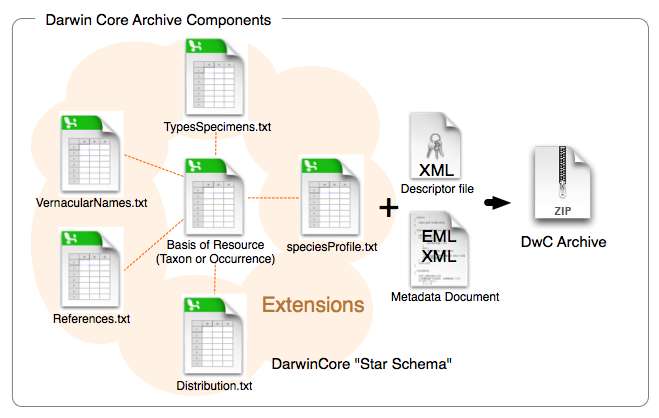
\includegraphics[width=\textwidth]{Chap5/figures/dwca.png}
    \caption{A Darwin Core Star Archive \cite{wieczorek2012}}
    \label{dwca}
    \end{figure}

Listing \ref{dwc:set} shows the comma-separated central file (Basis of Resource) containing the core details of the observation, i.e. the animal observed, and the column headings map to the descriptor file. Other linked files are typically linked by the unique ID of the observation, containing information that extends the observation and provides further context.

\noindent\begin{minipage}{\textwidth}
\lstinputlisting[caption=Darwin Core Occurrence Data, label=dwc:set]{Chap5/figures/dwc_arch/set.csv}
\end{minipage}


% Ecological Metadata Language (EML) is a metadata used by ecologists and the language is used to describe projects and those involved. This file acts as a form of certificate and descriptor as to what the data is related to and who owns it. The XML file, shown in Listing \ref{arch:dwc:eml}, outlines a sample project and users involved in the project.

% \lstinputlisting[language=XML, firstline=0, lastline=21,breaklines=true,label=arch:dwc:eml,caption=Darwin Core: EML.xml]{Chap4/listings/dwc_arch/eml.xml}

% The core file, \textit{meta.xml}, shown in Listing \ref{arch:dwc:meta} lists the files that contains the actual sensed data, as well as the terms used to describe it. Examples include: date, time, location, type of data, filename and species contained.

% \lstinputlisting[language=XML, breaklines=true,label=arch:dwc:meta,caption=Darwin Core: meta.xml]{Chap4/listings/dwc_arch/meta.xml}

% Data files contain the actual sensed data, based on how it is supported, and these files are linked in \textit{meta.xml}. For example, temperature readings or direct human sightings would be stored in a CSV file and linked, however, images or video would require the metadata to be store in a CSV file and a filepath would be referenced in the XML. The structure of the CSV file contains a header line that matches the terms in the meta file and each line would be an observation. The terms are linked to the Darwin Core glossary so the archive can be validated and processed by a DwC archive reader.

All of these files are then archived and sent as a ZIP folder throughout the network. If the sensed data is media based, then the media is included as well. Sofwtare libraries to process DwC archives are included on both DP and DA nodes.

Darwin Core is suited to K-HAS because its use in scientific observations matches our motivating scenario and the archive can be easily created by a DC node, as it does not require any heavy processing and all of the files are commonly used formats.
	
	\subsection{Middleware}
	The knowledge-processing capabilities of DA and DP nodes are the same and this is part of what makes K-HAS different from most other WSNs; both types of node run the sensor middleware, but each for different purposes. DA nodes use the middleware for administrating the network, receiving and archiving sensed data and allowing users to provide classifications. DP nodes use it for the receiving, sending and controlling the flow of processing of sensed data before it is passed on.
	
	Existing suitable middlewares have been detailed in Section \ref{sec:middleware} and our requirements for K-HAS were partially determined by the expertise of the users in our motivating scenario. Below is a list of our three core requirements:
	\begin{description}
		\item[Portability] Heterogeneous WSNs utilise nodes with different architectures and capabilities, if middleware is to be used on the nodes it must be able to run on these varied devices. 
		\item[Usability] Users of K-HAS should not be expected to have knowledge of computer science or the underlying architecture, this network should be usable by almost anyone. The same must be said for the middleware as well.
		\item[Extensibility] A closed-source middleware can be used, but it must then support all sensor nodes and data types, as well as receive regular updates. Open-source, or extensible, middleware can be used to add support for newer nodes.
	\end{description}
	
	GSN is a Java-based open-source middleware. New generic sensors can be added through XML files, while more complex sensors can be added through custom Java classes. GSN is covered in more detail in Section \ref{sec:GSN}. Because GSN can run on any architecture that supports the Java Virtual Machine (JVM), it meets our portability requirements and the web interface to provide administrative functionality makes it usable by those without any domain knowledge. Finally, the ability to add new sensors through XML means that it can be extended by almost any user of the network with very little guidance.
		
	\subsection{Knowledge Capture}\label{arch:kc}
		GSN is packaged with a web interface that allows users to see all nodes deployed and view the latest sensed data received. The web interface is targeted towards users with domain expertise and has limited functionality focussed towards sensor administration. However, it does make GSN accessible by more than one computer, as well as a variety of different architectures. For example, the admin webpage could be accessed on the machine that runs GSN, or from a tablet computer connected to the same network. We used the same approach to develop a web-based tool that provides access to all sensed data, as well as a simple interface for performing tasks, such as uploading new rules or updating the location of nodes.
		
		All sensed data is read from a MySQL database and users can view the metadata from each observation, such as location, date, time and temperature, as well as the data itself. From this, users are able to classify the data based on their role. Shown in the ontology in Chapter \ref{chap:ont}, K-HAS uses roles to control active projects and classifications; there are administrators and researchers. Researchers are involved in projects and receive notifications when relevant data has been received. They have access to the web interface and can vote on classifications for sensed data. Administrators lead projects and can create/complete them, but they also have the ability to finalise classifications. K-HAS follows a knowledge hierarchy (Figure \ref{arch:kno:hier}), with administrators at the top and DC nodes at the bottom. While there are more DC nodes in the network, their knowledge bases are more limited and classifications are trusted less than classifications made by DP nodes. Although there are fewer DP nodes, their knowledge bases are more detailed. Researchers and admins do not share a level on the knowledge hierarchy because we assume that administrators would be more experienced domain experts. For example, researchers could be students at Danau Girang, whereas an admin would be a professor with more experience. When an administrator makes a classification, all prior classifications are ignored and the feedback loop protocol is used to update nodes.

		\begin{figure}[!h]
			\centering
			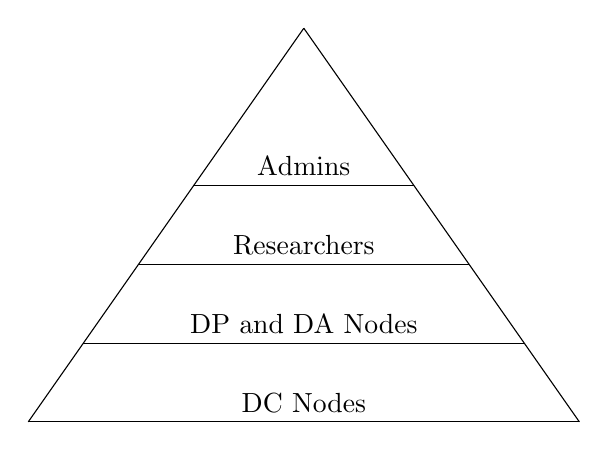
\begin{tikzpicture}

			\def \h {5};
			\def \f {.7};

			\foreach \y in  {0,1,2,3} {
			    \def \w { \h*\f-\y*\f };
			    \def \v { \y*\f-\h*\f };
			    \draw (\v,\y) -- (\w,\y);
			}

			\draw (-\h*\f,0)  -- (0,\h);
			\draw (\h*\f,0)  -- (0,\h);
			\node at (0,0) [above] {DC Nodes};
			\node at (0,1) [above] {DP and DA Nodes};
			\node at (0,2) [above] {Researchers};
			\node at (0,3) [above] {Admins};
			\end{tikzpicture}
			\caption{Knowledge Hierarchy for K-HAS}
			\label{arch:kno:hier}
		\end{figure}
		
		Figure \ref{kc:loris} shows an observation where users can vote on the contents. An administrator can then confirm that classification and prevent further votes from being cast. This type of moderation means that it does not have to be specialists voting on sensed data that cannot be classified by DP nodes.
		
		\begin{figure}[h]
		\centering
		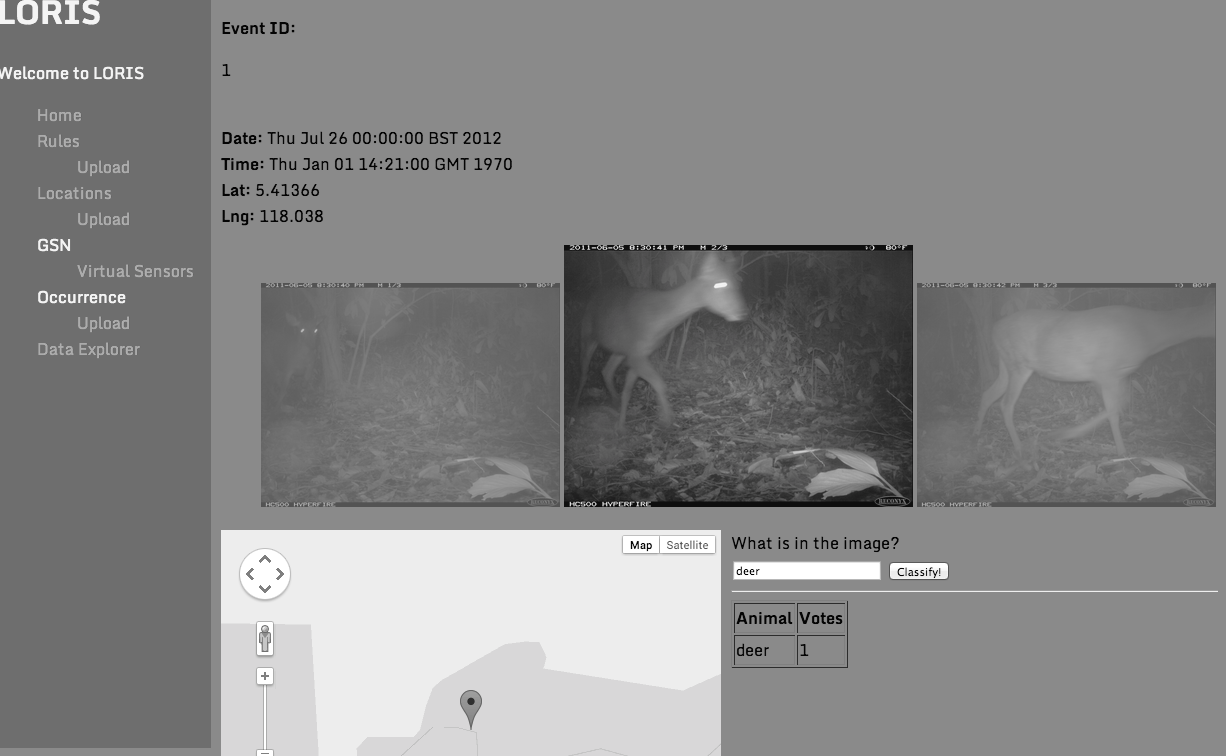
\includegraphics[width=\textwidth]{Chap4/figures/loris}
		\caption{Web Interface for Observations}
		\label{kc:loris}
		\end{figure}
		
		Viewing data for new observations is useful for gaining classifications and alerting members of a project, but viewing older sensed data allows patterns to be identified in order to create new rules. Figure \ref{kc:loris_data} shows a map of all deployed nodes in the area surrounding the field centre in our motivating scenario. When users select a node, a table is populated with all of the classified observations that it has captured; this can then be used to extract patterns from the data and create rules. For example, the two observations of the Malay civet are only seen late at night, if further observations also showed this, then we could create a rule defining the active hours of the Malay civet and, potentially, list days that it is likely to pass. These rules can then be written and uploaded to the knowledge base.
		\begin{figure}[h]
		\centering
		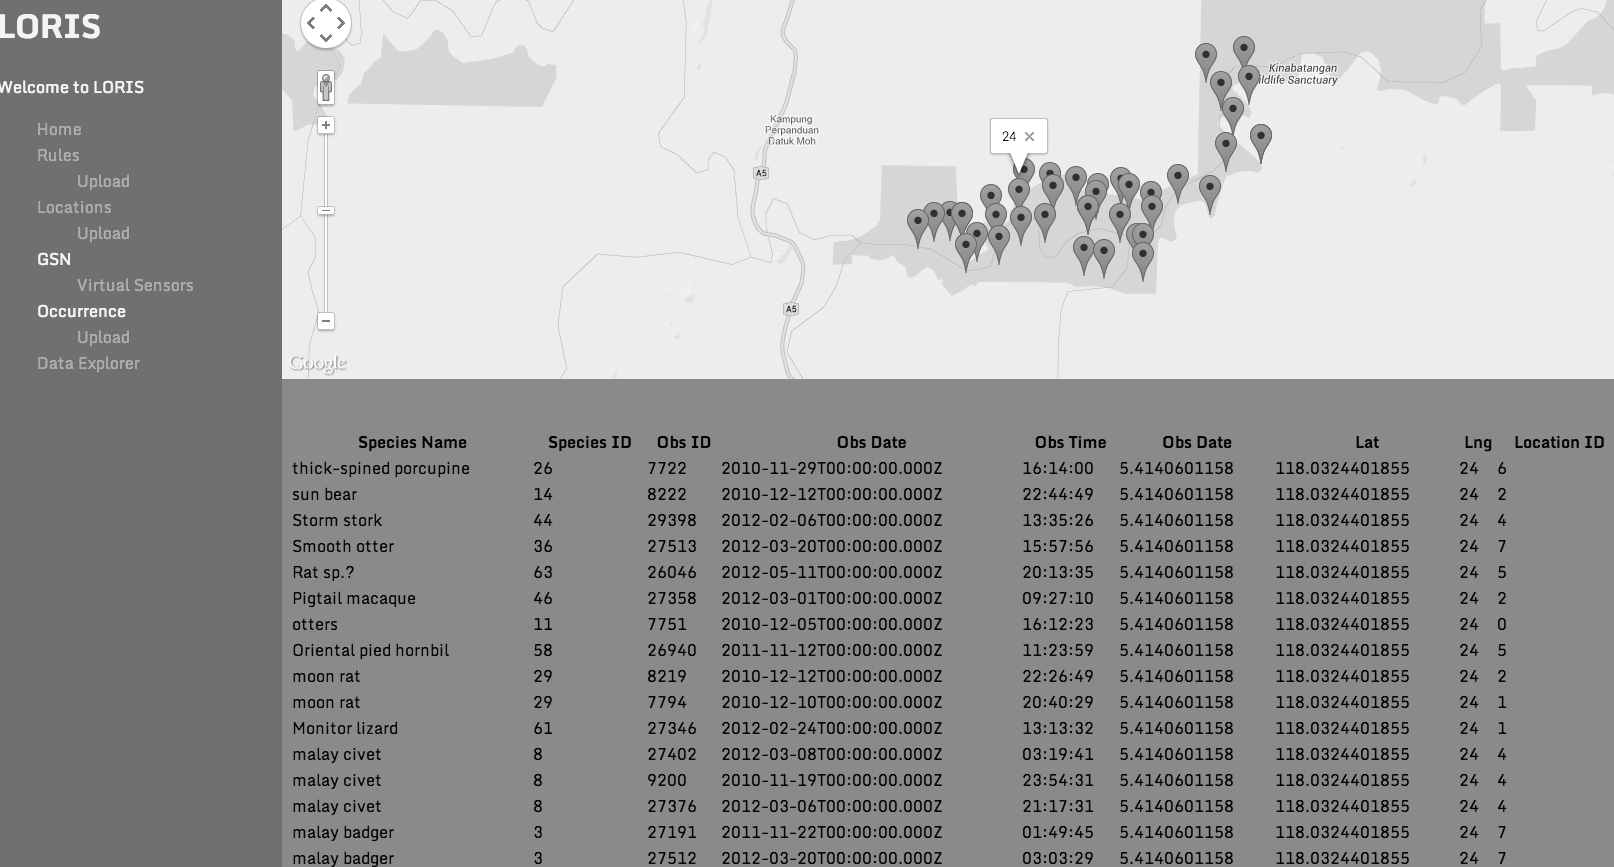
\includegraphics[width=\textwidth]{Chap4/figures/loris_data}
		\caption{Web Interface for Classified Sensed Data}
		\label{kc:loris_data}
		\end{figure}

		
	
	\subsection{Knowledge Base}\label{arch:kb}
	%Discuss drools here and the API developed for access to it from Sitesy.
	The Drools rule engine is a Java-based engine that uses forward chaining inference for the processing of rules \cite{proctor2005drools}, which means that rules are used to make meaningful inferences about data. Unlike DC nodes, which have limited knowledge processing capabilities, Drools is able to chain rules together and a rule that may not have been triggered at the start of processing may be triggered later if another inference is made. For example, a rule that is specifically for small mammals may not be triggered until an inference has been made that the image may contain small mammals based on the time and location of the observation.
	
	Drools is able to dynamically update its knowledge base, adding rules and firing them on observations that have already been loaded, as well as newer ones. This allows DP nodes to adapt to new rules and local knowledge whilst they are deployed. The use of \textit{drl} files use a mixture of Drools and Java syntax to define rules, allowing them to modify, or create, Java objects. For example, a rule could be triggered on the receipt of sensed data and create a DwC object from the received data, process it and perform checks on the result that would trigger different rules based on that result. This is one of the main reasons we chose Drools, as it can work with GSN and DwC Java objects, as well as the ability to run on any architecture that supports Java.
	
	The functionality of Drools is extensive and the engine is very powerful, however, it does require specialist knowledge to use and manipulate rules. Using a custom developed Drools web interface , detailed in Section \ref{arch:kc}, we created a simplified interface that uses a custom REST API for Drools, allowing users to create sessions, add rules, load data and fire rules, returning the output to the interface. Users can view, and load, existing drl files, shown in Figure \ref{kc:loris_drl}. 
	
		\begin{figure}[h]
		\centering
		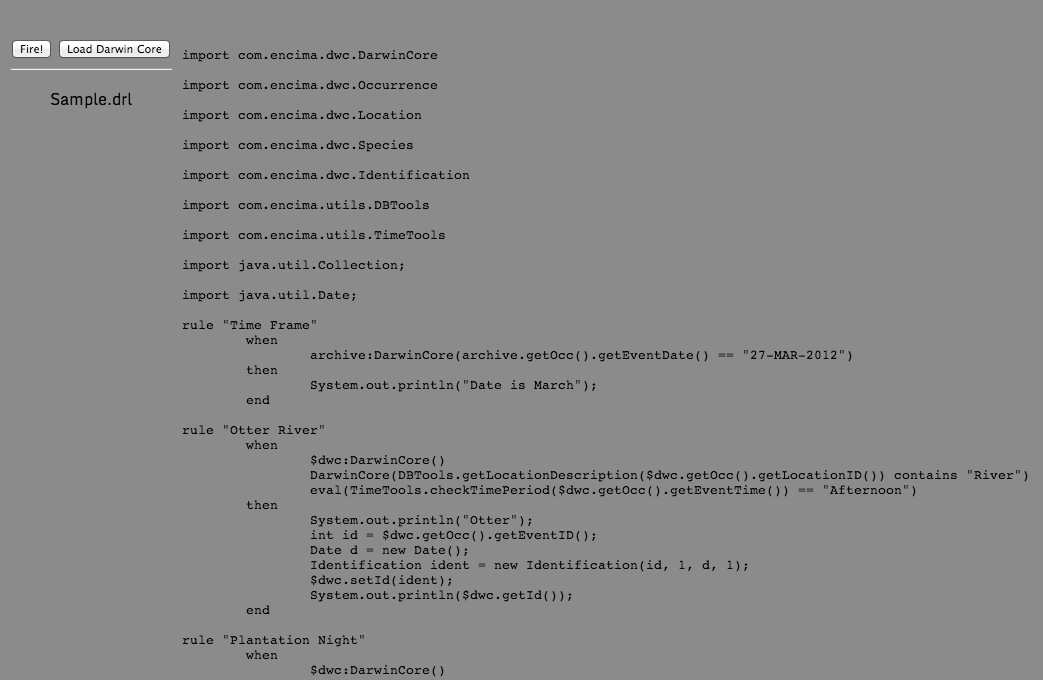
\includegraphics[width=\textwidth]{Chap4/figures/rules}
		\caption{Web Interface for Drools Operations}
		\label{kc:loris_drl}
		\end{figure}
	
	Once a file has been selected, users can view the rules and use the controls on the webpage to perform common operations. The \textit{Load Darwin Core} button loads all DwC archives that are stored in the MySQL database into the current Drools session and the \textit{Fire} button runs all loaded rules on the loaded data. If any of the rules trigger, then the output is presented to the user in the same page, allowing them to act on the results. For example, the location of observations could provide a narrowed down list of potential classifications, allowing an administrator to remove votes that do not match the list.
	
	Currently, these implementations have been developed for our motivational scenario, but much of these tools are general enough to be repurposed in order to apply to a variety of different WSNs. The Drools API can be used for any kind of sensed data and the web interface would require minor changes to be extensible.

	\subsection{Routing Protocol}\label{arch:routing}
		The routing protocol we have selected for K-HAS is not fixed for every deployment but, from our research, we modified the commonly used Mininum Cost Forwarding Algorithm (MCFA), outlined in Section \ref{bg:rp:mcfa}, as it allows for changes in the topology of the network and does not require every node to have a global view of the network.

		On deployment of all nodes, a DA node sends out a packet containing the number zero, representing the number of hops to the DA node. Nodes in range receive the packet, store it along with the identifier of the originating node and then send it once it has been incremented by one. The next nodes receive that packet and do the same until the edge of the network is reached. If a node has a number stored that is higher than the one it receives then it is replaced and sent on until the nodes at the edge of the network are reached.

		When a node wants to send data, it queries neighbouring nodes and sends to the node with the lowest hop count to the root. We modified this to run in accordance with our tiered architecture as we expect the topology to remain the same for much of the deployment.

		In MCFA, nodes do not store path information and messages are broadcast to all nodes when they are sensed.

		Firstly, our protocol runs in two modes: configuration and running. During the configuration mode, we use MCFA. Whereas MCFA does not store path information, we use the method desribed above to store both the hop count and the nearest neighbour. This process is carried out until all nodes of the network have a hop count (and neighbour) and a final pass is made by all nodes to find, and store, their neighbour with the lowest count. The main difference is that, unlike MCFA, not all nodes process all packets. If a packet originates from a DA node, then it is only stored by DP nodes but DP node packets are stored by both DC and DP nodes. DC nodes store it and send all data through their nearest DP node and DP nodes store other DP neighbours to delegate processing to, should a situation arise where they have too much data to process and cause a bottleneck. Configuration mode can then be run at a set interval throughout the deployment of the network, or initiiated manually.

		Whilst in running mode, nodes do not query for the neighbour with the lowest hop count, or broadcast the sensed data to all nodes in range, they send to the node stored as their nearest neighbour. If that fails, then a query is sent out to find other available nodes in range and then sent to the one with the lowest hop count. If the nearest neighbour node is unavailable for more then three attempts, then it broadcasts a request to run the configuration mode again.

	
	\section{Walkthrough}\label{arch:walk}
		In this section we will explain the steps involved in the capture, and processing, of an observation when using the K-HAS architecture. Each tier is responsible for performing different actions upon the observation to ensure it is received by the DA node with an inference as to what it may contain.
		
		\subsection{Scenario}\label{arch:scen}
			This walkthrough will use our motivating scenario and the type of sensed data will be images of animals in the Malaysian rainforest. In this example, we have a collection of wildlife cameras, with nodes attached to them, deployed in the forest. Projects for the rare clouded leopard and sun bear are currently active at Danau Girang. The clouded leopard is a nocturnal carnivore that uses existing paths and hill trails to travel through the rainforest and the sun bear is the smallest bear in the world and sightings are rare. It is also nocturnal and claw marks can be seen on trees that they have climbed. All of this information has been encoded onto the DP nodes and DC nodes know that images taken at night will be of a higher priority, as well as to prioritise further images at night from DC nodes that are deployed on ridges or existing trails.

			In order to explain the K-HAS architecture, we need to show the planned topology for the network in Danau Girang, which is based on the positions of the cameras in 2010. Figure \ref{topol} shows a section of the proposed topology around the field centre, with the rest of the network spreading out along the river on both sides. The triangle icon shows the location of the DA node (at the field centre), with DP nodes (square icons) placed near the DA node because of the poor range of Wi-Fi (Section \ref{tech:wifi}). Circle icons represent the DC nodes and they link to the nodes with the fewest hops to a DA node, as long as that route includes a DP node. 

			\begin{figure}[!t]
			\centering
			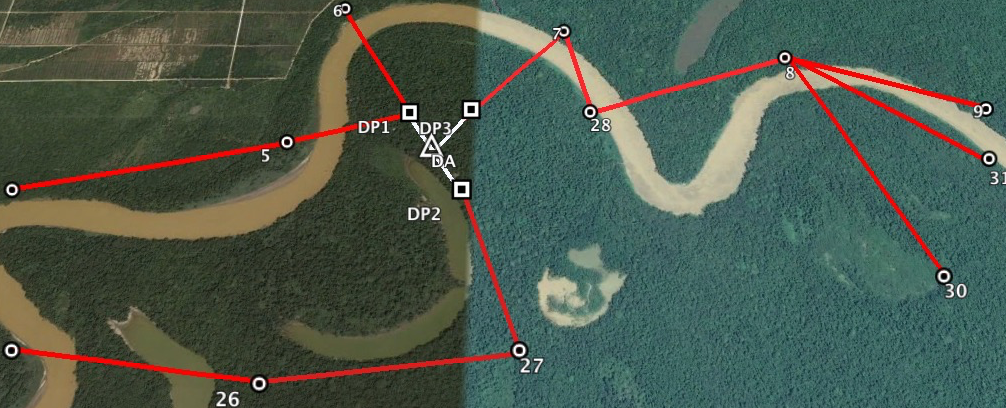
\includegraphics[width=\textwidth]{Chap4/figures/topology}
			\caption{Section of Proposed Topology for K-HAS in Danau Girang}
			\label{topol}
			\end{figure}
			
		\subsection{Data Collection}
			A DC node is deployed along a ridge in the rainforest and consists of a wildlife camera with a wireless node attached. At 0200, the infra-red sensor detects movement and the camera triggers a set of 3 images to be captured. The DC node creates the DwC archive for the observation. Terms that describe the observation, such as time, date, species identified and location, are added to the meta.xml file and links to CSV files that contain the data for each term. Any field that can be completed, such as time, location and date, are added to the set.csv file. A separate CSV file is created that holds the filename of each image that was taken. The image is shown in Figure \ref{cl2}.
			
			\begin{figure}[!t]
			\centering
			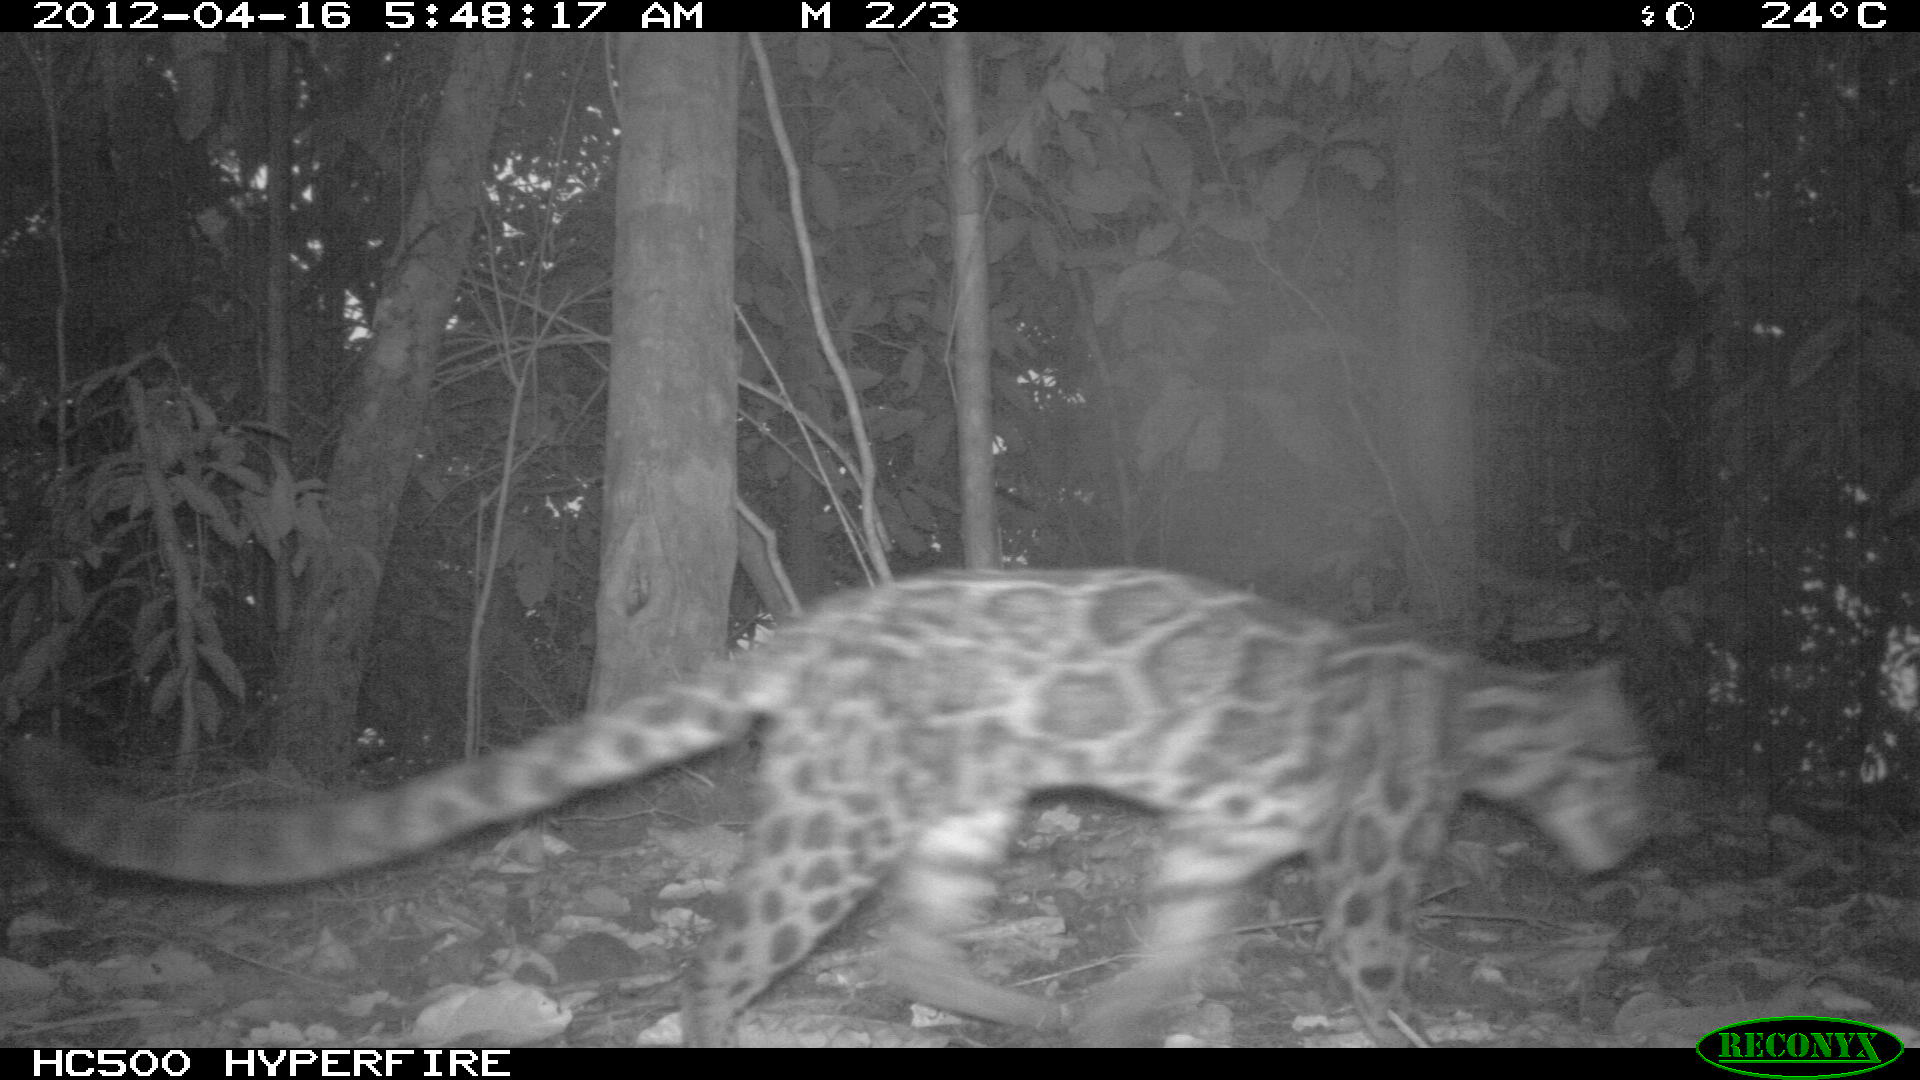
\includegraphics[width=\textwidth]{Chap4/figures/leopard2.JPG}
			\caption{clouded leopard Image Capture}
			\label{cl2}
			\end{figure}

			\begin{figure}[!t]
			\centering
			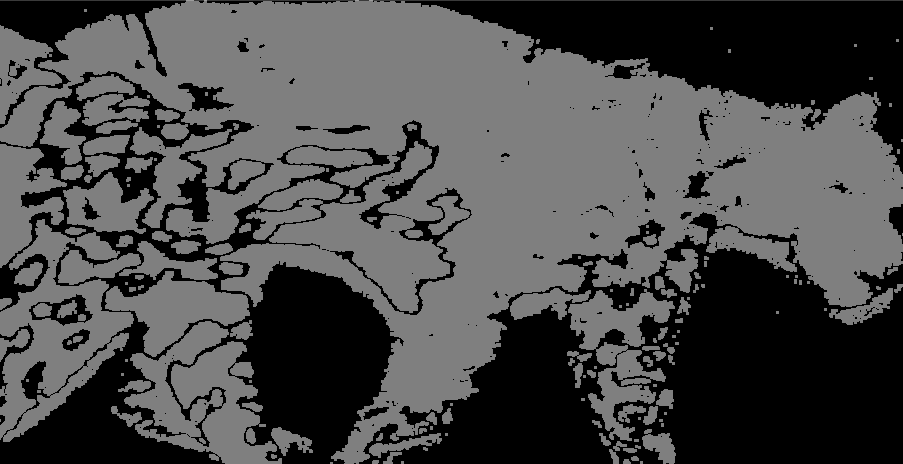
\includegraphics[width=\textwidth]{Chap4/figures/leopard_proc}
			\caption{Processed Image of clouded leopard}
			\label{clproc}
			\end{figure}
			
			The DC node runs its rules on the metadata of the images and infers that the image may contain a clouded leopard, this is because the image was taken in the early hours of the morning and the camera is deployed on a ridge. DC nodes run simple, non-chaining rules based on the file metadata and details about the node, such as location, but these rules are fixed from the time of deployment and are not updated until the network is redeployed. When bandwith is restricted, DC nodes us a queue to prioritise both their own observations and those receivied from other nodes. Observations marked as interesting are moved to the front of the queue and any others are sent afterwards.
			
			The inference is included in the archive and is compressed. The node then sends it through every DC node between the originating node and the DP node assigned. To achieve the long range communications in the forest, Digimesh is used; the low transfer rate does mean that an archive can take several minutes to send but it allows for a range of up to 1km.

	\subsection{Data Processing}			
			The DP node receives the observation and it is unzipped and processed by the Darwin Core library. If the data has been preprocessed by a DC node and marked as interesting, then the processing is prioritised, otherwise it is added to the queue. In this case, the DC node believes the observation is interesting and may contain a clouded leopard, so it would be processed before other observations that may be queued and not marked as interesting. The images are read from the filenames provided in the CSV and processed using two methods. The EXIF tags in the image are extracted and the images themselves are processed using the Open Computer Vision (OpenCV) library. A unique feature of the DP node is that it uses two radios to allow links to both DA and DC nodes. DC nodes send archives using Digimesh, to achieve long range communcation, and DA nodes use Wi-Fi, to provide a faster transfer rate than Digimesh and a more standard method that allows other devices to connect, such as mobile phones or laptops.
			
		\subsubsection{EXIF}
			EXIF (Exchangeable Image Format) tags are written to images at the time of capture. Examples of these tags can be time, date or camera serial number. The capabilities of the camera do affect how detailed the EXIF is, for example, a camera with GPS capabilities will enrich the image with the location. 
			
			Wildlife cameras have more functionality than common digital cameras, with details like moon phase, temperature and/or GPS location. Some devices even include the saturation, brightness and hue of each image. These capabilities allow the EXIF to be extremely detailed and this metadata can be used to find patterns in pictures that, when accompanied by local knowledge, assist with the classification of sensed data. 
			
			In this example, the knowledge base on the DP node is aware that clouded leopards and sun bears are nocturnal, but clouded leopards have previously only been seen when the temperature is between 30 to 35\celsius\ and only when the moon is not full. However, data on sun bear is not as complete and the knowledge base only shows that the bear is nocturnal and can be seen at any time of night in any area of the rainforest. The DP node identifies that the moon phase is not full and that the temperature is 32\celsius, from this it determines that the image could contain either animal and it cannot make a final conclusion.
			
		\subsubsection{Image Processing}
			Our Triton program, described in Section \ref{tech:sf:triton} is run on the set of three images. These images are converted to black and white and combined to build a background model for the complete set. The detected background is then removed and the final image is then searched for objects, where objects in the foreground will be shown with white pixels. The largest object is then found in the image and extracted to create a template, shown in Figure \ref{clproc}.
			
			Processed images of previously sensed images are stored on the DP node and associated with the confirmed classification, confirmed by a human or a node. Although the memory available on a DP node is typically around 32GB, this could easily fill in a matter of months if 3 full HD images were stored for every observation. Storing a single black and white template that contains a portion of the image is much more efficient and can still easily be associated with the classification made. The extracted image is then compared with the existing images, using the knowledge base to prioritise templates for comparison. In this example, nocturnal animals are prioritised and especially nocturnal animals with active projects associated. If the DP node has received an observation from the same DC node recently, then it will check for a classification on that and check for a match there first.
			
			This observation is the first trigger from the DC node in the past few hours, so there are no recent classifications. However, processing of the metadata showed that the image was taken at night, so the DP node uses its knowledge base to match the images to templates of nocturnal animals first. Triton then finds a match to an existing template of a clouded leopard and completes its classification.
	
		\subsubsection{Classification}
		The metadata processing of the image shows that it could be any nocturnal animal that is known to come out when the moon is not full and the temperature is 32\celsius. This is not a complete classification but the image processing has found a match. These findings are written into the set.csv file of the DwC archive (Listing \ref{dwc:set}), using the identifier of the DP node as the `person' that identified the image and the scientific name for the clouded leopard as the species identified in the image. The archive is then zipped and sent on to the DA node, sending observations of interest first and delaying observations that have been found to contain nothing of interest.
			
	\subsection{Data Aggregation}		
			Upon receiving a DwC archive, it unarchived and processed by Darwin Core libraries, called by the middleware running on the node. The resulting archive is then inserted into a MySQL database and the files themselves are stored in a directory that maps to the DC node that captured the original observation. At the field centre, three users of the system have subscribed to updates for observations of clouded leopards.
			
			As the archive is processed by the library, the species is extracted and this triggers a rule to notify the subscribers. The rule then queries the database and finds their preferred method of communication. In this case, one is a lecturer and wants to be emailed while the two remaining are students and want to be notified via Twitter. An email is generated that contains the time, location and content of the observation, with the images attached, and sent on to the lecturer. The students are sent a short tweet that tells them a clouded leopard has been spotted and a link to the middle image in the sequence is provided; the middle image is used because local knowledge has shown that it is the most likely to contain the full subject in the image. In order to maintain privacy, a `direct message' can be sent on Twitter so this the message is not public.
			
			The middleware on the node supports a web interface to allow users to perform administrative functions on the network, such as deploy a new node, on top of this there is a custom made website that shows all observations for every DC node. This allows users to log on and classify the images. In this case, the lecturer receives the email notification, reviews the attached images and clicks on the link to access the website to inform the DP node that the classification was correct. Due to the administrator position the lecturer has on the system, he is able to stop any users voting on the image and to simply confirm the classification.
			
			If there was no classification, then users would be able to vote on the contents and use the classification with the highest vote, or the classification made by an administrator. Once a classification has been made, it is stored in the database and written to the archive. This triggers the DA node to send that classification on to the DP node that sent the original archive. In this case, the DA node informed the DP node that it has been confirmed as a clouded leopard and the DP node then stores the extracted image in the directory of clouded leopard templates, to assist with future classifications. This updated template causes the rule base of the DP node to be updated so similar data processed in the future would be correctly identified. The longer the network is deployed, the more knowledge DP nodes gain and the more accurate their classifications can be. For example, a change in season could cause a new, previously unknown animal to migrate to the rainforest. With human assistance, the animal can be identified and determined whether it is of interest. This knowledge can then be stored and sent on to DP nodes to prioritise and classify correctly the next time that it is captured. The feedback loop protocol is currently only a design and has been minimally implemented as a proof of concept.
					
	\section{Conclusion}\label{arch:conc}
		In this chapter we have explained the architecture we have developed to allow knowledge to be encoded and utilised within a wireless sensor network. Using tiers of nodes, with varying levels of knowledge-processing capabilities, we can process observations within the network and deliver data that has, where possible, already been classified. Working as more of a subscribe-push method, users do not have to check a DA node for new data, instead it is sent to them if it has been found to be part of a project they are subscribed to. If not, then the data is accessible to all users of the network through a web interface.
		
		One of the key features of K-HAS is that it is not a static deployment. The knowledge that the network holds at the time of deployment will rarely be the same as the knowledge held after a few months. Humans enrich the existing knowledge base and the nodes are able to make inferences about the data they are sensing, improving their classifications the longer they are deployed.
		
		In Chapter 6, we explain how we implemented a variation of K-HAS in our motivating scenario and Chapter 7 shows our evaluation of the K-HAS architecture, but Chapter 5 will first outline the development of an ontology to support the architecture described here.
		
			
			
			
			
			
			
			
			